\chapter{Literature Review}

\begin{enumerate}
	\item [Technology] background 
	\item Depth Sensor technology + How Kinect works
	\item Point cloud map
	
	\item [Coding] references/Getting started
	\item Code references and and blog posts? 
	\item Previous example
	\item Hand Example
	
	\item [Mathematics] Used
	\item Papers on ellipse circumference
	
	\item [Improving] Accuracy
	\item Skeleton Joints filtering
	\item Error Model
	
	\item [Further] developments
	\item Augmented reality paper
	
	\item [Imaging] Processing Background
	\item Basics of an image - RGB
	\item Matlab
	\item Camera Model
	
	\item [Uncertainty] Measurements
	\item Gaussian 
	\item Triangular
\end{enumerate}

\section{Literature Guide}
\subsection{Getting Started}

\subsubsection{Non-Contact Human Body Parameter Measurement Based on Kinect Sensor \cite{nonContact2017}}

\paragraph{Overview}
This journal article provides an adequate base to understand many techniques used during this project. In the article, a similar project is explored in terms of using a Kinect to determine various personalized measurements. This includes measurements such as height, shoulder length, other key limb lengths and front perimeter measurements for the chest, stomach and waist. All of the work done in this article is similar to the work done in the initial stages of this project. The article also provides useful contextual information regarding the current use of this technology and background knowledge regarding the inner workings of the Kinect. 

\paragraph{Relevance}
The main contribution of this article was the background information it provided, together with the validation of certain aspects of the experiment methodology: 

\subparagraph{Background Theory}
This article provides a summary and overview of the process the Kinect utilises to retrieve data about a detected human. It explains the different sensors the Kinect posses, together with a basic understanding of the internal process required to track a skeleton and return information such as "Joint" position etc. This is explained in more detailed in Section \hl{(Reference to Middleware)}. It also provided an explanation of how pixels in the image plane are converted to real world positional points using information from both depth and colour frames. This is also explained in detail in Section \hl{(Depth - real conversion)}.

\subparagraph{Methodology}
This article was found after an initial strategy for calculating measurements was created. However, it served as a validation of the methods used, specifically with regards to using the Pythagorean Theorem in 3D space to calculate distances and for calculating the error between actual measurements and measurements obtained using the Kinect. These methods and the relevant equations are explained in Section \hl{(Measurement - Pyth + error)}. A method was also suggested for the calibration of results to improve their accuracy. However, this technique was not employed in this project. Reasons for the exclusion are given in Section \hl{(Design - No calibration or correction)}

\subsubsection{Real-Time Hands Detection in Depth Image by Using Distance with Kinect Camera \cite{handDetection2015}}

\paragraph{Overview}
This journal article explored various techniques to improve hand detection using a Kinect. The main focuses were in the areas of background removal, noise removal and feature extraction. Traditional image processing techniques require a large amount of processing power and often produced ambiguous results, with regards to feature extraction, and were prone to noise. Introduction of the Kinect allowed for the use of depth data to reduce the computational power needed and to improve the accuracy of the results. A large section of the paper was dedicated to "Shadow Removal", which is the process of removing depth data unavailable due to an object obstructing the emitted Infrared Rays. "Shadow" was determined to be a significant source of noise in the depth data and its removal improved the accuracy of the system.    

\paragraph{Relevance}
This article was very specific to the detection of hands and therefore its use was limited. However, valuable insights were gained regarding the "Shadow Removal" and Background Removal processes implemented \hl{(Classifier Maybe)}:

\subparagraph{Shadow Removal}
The intricacies of Kinect in creating a depth image using its IR Emitter and IR Camera were explored in more detail. This further expanded on the inner workings of the Kinect and contributed to Section \hl{(Depth Image Creation - Kinect)}. Additionally, this brought attention to a significant source of noise in the depth image and provided a method to improve the accuracy of measurement results. This method is explored in Section \hl{(Rec - Noise Removal)}

\subparagraph{Background Removal}
This article detailed a method of Background Removal that did not utilise the BackgroundRemoval API available in the Kinect for Windows SDK. This method provides an alternative method for background that could be investigated if the BackgroundRemoval API does not provide the desired results. This is explored further in Section \hl{(Rec - Background Removal)}

\subsubsection{A Real Time Virtual Dressing Room Application using Kinect \cite{virtualDress2012}}

\paragraph{Overview}
This report details and explains an approach used to create a virtual dressing room. The end result was an application that allowed a user to see what clothing would look like by augmenting it onto their body. This was executed in a three part process of user extraction, user tracking and clothing mapping. A Kinect sensor was used to extract the user from the background using depth images and user information. The Kinect was also used to track the skeleton of the user and create a coordinate system on which the virtual clothing could be mapped. Lastly, information including joint orientation and key body lengths were used to augment the clothing model onto the body.  

\paragraph{Relevance}
This report details and explains a possible extension on this project that would be very useful in a production level solution. 

\subparagraph{Augmented Reality}
The virtual dressing room proposed in the report is foundational solution using augmented reality and requires further work and research in itself. However, once it is improved to a level sufficient for implementation, it would significantly improve the customer experience. This is envisioned to be used after the customer uses the system, proposed in this report, to determine their full body parameters. The customer would be able to use the virtual dressing room to get an accurate understanding of how different clothes would look on them, without needing to physically try them on. This is expanded on in Section\hl{(Rec - Virtual Dressing Room)} 

\subsubsection{Performance Evaluation of the 1st and 2nd Generation Kinect For Multimedia Applications}

\paragraph{Overview}

\paragraph{Relevance}

\subparagraph{Background Theory}

\subparagraph{Component Selection}




Definitions!!!!!!!!!!!!!!!!!\\
Accuracy\\
Precision\\
Kinect\\
Volunteer\\
Operator\\
IR - Infrared Rays\\


When writing your review start of with the general concepts and move to the more specific aspects
explaining the necessary theory as you go. This section is NOT a copy and paste from others work or a
rewrite-but-change-one-word section. I suggest you read all your material, and then put it down and
write this section, referring back to the work only when you need to check something.

See your PCS textbook for more details on how to write a literature review.

If you include a figure or a table in your text please see the example in Fig. \ref{fig:model} as to how to caption it.
Please make sure that all text in your figures is readable and that you reference your figures if they are
from another source.

\begin{figure}[ht]
\centering
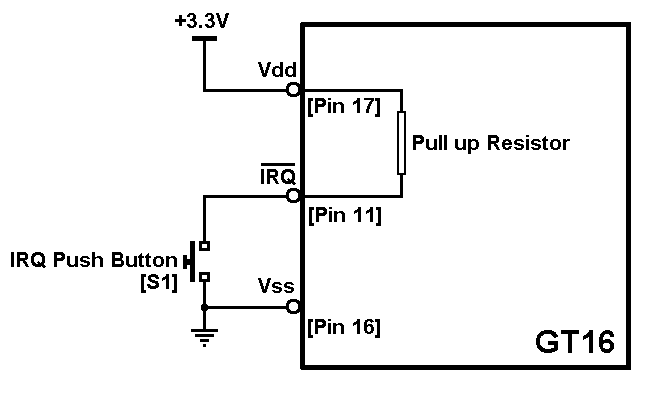
\includegraphics[width=0.7\textwidth]{model.png}
\caption{A block diagram illustrating the connections to the IRQ pin on the MCS08GT16A microcontroller (Please
note that your headings should be short descriptions of what is in the diagram not simply the figure title)}
\label{fig:model}
\end{figure}

